
\chapter{Conclusiones}

FIXME

\section{Conclusiones personales}

Este proyecto me ha supuesto muchas cosas a nivel personal y profesional. He
aprendido mucho sobre esta incipiente área que es la Web Semántica; tengo la
suerte de contar con dos directores de proyecto (José Emilio Labra y Diego
Berrueta) que grandes expertos en la materia y me han ayudado en todos estos
meses.

Además me ha brindado la oportunidad de un nuevo lenguaje de programación al
que hacia tiempo le tenía ganas: Python.

Desde el punto de vista ético para mi era muy importante saber que las horas
invertidas en este proyecto no se \emph{morirían} en las polvorientas estanterias
de la biblioteca. Por eso desde eso desde el principio y en todo momento el
proceso de desarrollo de todos los componentes de este proyecto ha estado
disponible en el subversion de Berlios\footnote{\url{http://swaml.berlios.de/wsvn}}.

En estos meses he liberado media docena de versiones de SWAML. Quizás el recorrido
termine aquí, o quizás no. No sé si yo continuaré desarrollando SWAML o si a alguien
le parecerá interesante para continuar el trabajo que yo he comenzado; pero el caso
es que el software liberado ahí seguirá para cualquiera que sea el uso que alguien
le quiera dar.

\section{Conclusiones sobre la aportación de SWAML}

FIXME(SIOC, etc)

\section{Trabajo relacionado}

FIXME(¿la idea de swaml a que más podría aplicarse?)

\section{Conclusiones sobre el software utilizado}

Ha sido mucha la diversidad de software (complidores, bibliotecas y herramientas)
utilizado para la realización de este proyecto. Nótese que todo él se ha podido
desarrollar utilizando únicamente \emph{software libre}.

\subsection{Python}

FIXME

\subsection{Bibliotecas\label{sec:conclu:bib}}

FIXME(¿más?)

\subsubsection{RDFLib}

RDFLib\footnote{\url{http://rdflib.net/}} FIXME

\subsubsection{dom.xml}

dom.xml\footnote{\url{http://docs.python.org/lib/module-xml.dom.html}} FIXME

\subsubsection{PyGTK}

FIXME

\subsection{Herramientas}

FIXME

\subsubsection{Subversion}

Se han hecho 458 commits (FIXME: actualizar antes de imprimir)...

\begin{figure}[ht]
	\centering
	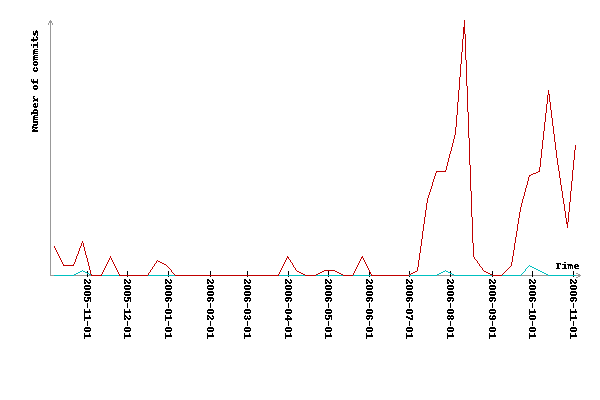
\includegraphics[width=12cm]{images/svn-stats.png}
	\caption{Estadísticas del subversion de SWAML}
	\label{fig:svnStats}
\end{figure}

\subsubsection{Autotools}

FIXME

\subsubsection{PyDev}

PyDev es un plugin para Eclipse FIXME

\subsubsection{Ant}

FIXME

\subsubsection{Gazpacho}

FIXME

\subsubsection{SWOOP}

Existen varios editores libres para ontologías OWL:

\begin{itemize}
  \item Protégé\footnote{\url{http://protege.stanford.edu/plugins/owl/}}
  \item SWeDE\footnote{\url{http://owl-eclipse.projects.semwebcentral.org/}}
  \item SWOOP\footnote{\url{http://www.mindswap.org/2004/SWOOP/}}
\end{itemize}

Los dos primeros no son más que plug-ins para dar soporte a OWL en dos 
frameworks. Y el tercero es un editor pensado y desarrollado explicitamente
para trabajar con OWL.

Después de las pruebas realizadas, SWOOP resultó ser una herramienta más sencilla,
comoda de usar y potente que las otras dos.

\begin{figure}[ht]
	\centering
	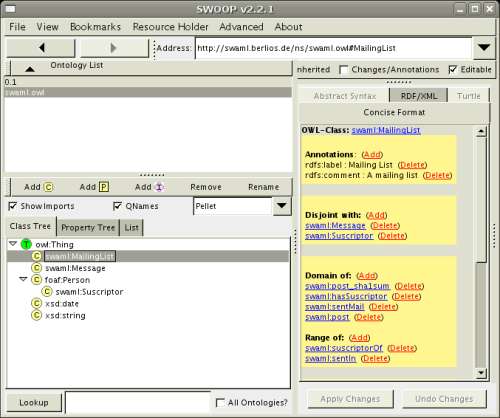
\includegraphics[width=11cm]{images/swoop.png}
	\caption{SWOOP editando la ontología de SWAML en OWL DL}
	\label{fig:evoWeb}
\end{figure}

Alguna de las caracteristicas más interesantes de SWOOP son:

\begin{itemize}
  \item Interfaz de usuario hypermedia similar a la de un navegador convencional, 
	con elementos (pestañas, marcadores, etc) que hacen la interfaz más 
	amigable.
  \item Soporte de depuración de la ontología.
  \item Cliente para hacer razonamientos sencillos con Pellet.
  \item FIXME
\end{itemize}

Un problema común en todas estas herramientas de alto nivel para trabajar con
grafos RDF es el serializado del grafo a sintáxis XML. No por su corrección,
que la herramienta lo hace perfectamente, sino por su orden: es muy difícil
que al serializar queden todos los nodos en el mismo orden. Por tanto es muy
difícil conocer las diferencias entre distintas versiones con las herramientas
convencionales (principalmente \texttt{diff}).

\subsubsection{phpWiki}

FIXME

\subsubsection{Google Maps}

FIXME(KML)

\subsubsection{\LaTeX}

\TeX/\LaTeX FIXME

\paragraph{Kile}

\paragraph{JabRef}

\section{Lineas de futuro}

El trabajo realizado hasta ahora con SWAML no ha hecho sino empezar, abriendo las 
puertas hacia una linea de desarrollo que puede significar un foco importante
en cuanto a la publicación en formatos semánticos de todo el conocimiento contenido
en esas miles de listas de correo existentes por lo largo y ancho de la internet
actual.

Aunque puede que no se incluyan todas las existentes, estas on algunas de las lineas
que seria interesante el proyecto abarcara algún día:

\subsection*{Integración con Mailman}

FIXME

\subsection*{API para DIG}

Sería interesante disponer de una API en Python para utilizar razonadores DL que implementen 
el protocolo DIG\footnote{\url{http://dig.cs.manchester.ac.uk/}}. 

Existen ya API's similares en Java (dentro del framework
Jena\footnote{\url{http://jena.sourceforge.net/how-to/dig-reasoner.html}} o incluso en Haskell 
(implementada dentro del proyecto WESO\footnote{\url{http://weso.sourceforge.net/}}. Por eso 
sería interesante implementar el protocolo DIG en Python, y no sería una tarea
en la que nos encontraríamos en solitario\cite{PythonOWL}.

FIXME

